%! Author = Wiktor Rostkowski, Mateusz Budzisz
%! Date = 29/04/2024

\chapter{Projekt}
\label{ch:projekt}

\section{Wzorce projektowe}\label{sec:wzorce-projektowe}
W projekcie wykorzystano następujące wzorce projektowe:
\begin{itemize}

    \item \textbf{MVVM (Model-View-ViewModel)}: Wzorzec architektoniczny, który oddziela logikę biznesową (Model) od interfejsu użytkownika (View) za pomocą warstwy pośredniej (ViewModel), która zarządza stanem i logiką prezentacji.

    \item \textbf{MVC (Model-View-Controller)}: Wzorzec projektowy, który dzieli aplikację na trzy główne komponenty: Model (logika danych), View (interfejs użytkownika) i Controller (logika aplikacji).
    Pozwala to na lepsze zarządzanie kodem i jego modularność.

    \item \textbf{REST API (Representational State Transfer Application Programming Interface)}: Styl architektoniczny dla systemów rozproszonych, oparty na protokole HTTP, który umożliwia komunikację między klientem a serwerem za pomocą standardowych metod (GET, POST, PUT, DELETE).

    \item \textbf{Repository}: Wzorzec projektowy, który zapewnia warstwę abstrakcji nad dostępem do danych.
    Umożliwia oddzielenie logiki biznesowej od warstwy dostępu do danych, co ułatwia zarządzanie danymi i testowanie aplikacji.

    \item \textbf{Dependency Injection}: Technika polegająca na wstrzykiwaniu zależności do komponentów, zamiast tworzenia ich wewnątrz komponentów.
    Umożliwia to luźne powiązanie między komponentami i ułatwia testowanie oraz zarządzanie zależnościami.

    \item \textbf{Redux}: Wzorzec do zarządzania stanem aplikacji, szczególnie popularny w aplikacjach React.
    Opiera się na centralnym magazynie (store), który przechowuje cały stan aplikacji, oraz na akcjach i reduktorach, które modyfikują ten stan w kontrolowany sposób.

    \item \textbf{Observer}: Wzorzec projektowy, w którym obiekt (obserwowany) powiadamia inne obiekty (obserwatorów) o zmianach swojego stanu.
    Umożliwia to reaktywne programowanie i luźne powiązanie między obiektami.

    \item \textbf{Reverse Proxy}: Serwer pośredniczący, który przyjmuje żądania od klientów i przekazuje je do odpowiednich serwerów docelowych.
    Używany do zwiększenia wydajności, równoważenia obciążenia i poprawy bezpieczeństwa.

    \item \textbf{Bearer Token}: Metoda autoryzacji, w której token dostępu jest przesyłany w nagłówku HTTP\@.
    Umożliwia to bezpieczne uwierzytelnianie użytkowników i autoryzację dostępu do zasobów.

    \item \textbf{Service}: Pojęcie szerokie, odnoszące się do jednostki funkcjonalnej w aplikacji, która realizuje określoną usługę.

\end{itemize}

\section{Komponenty}\label{sec:komponenty}
W skład systemu wchodzą:
\begin{itemize}
    \item Internetowa aplikacja progresywna
    \item Backend zgodny ze standardem REST API
    \item Baza danych PostrgeSql
\end{itemize}

\section{Architektura}\label{sec:architektura}
System został zbudowany w architekturze monolitycznej, co oznacza, że wszystkie jego elementy i funkcjonalności są zintegrowane w jednym serwisie, zamiast być podzielone na niezależne moduły lub mikroserwisy.
System został wdrożony w chmurze obliczeniowej Oracle Ampere.
Aby uniknąć problemów z CORS (Cross-Origin Resource Sharing), wszystkie połączenia przychodzące z różnych źródeł są przekierowywane przez serwer Nginx.
Nginx działa jako reverse proxy, który odpowiednio kieruje ruch do właściwych komponentów systemu znajdujących się na serwerze.
Dzięki temu z perspektywy użytkownika wszystkie usługi systemu są dostępne pod tym samym adresem URL\@.
Dodatkowo, użycie Nginx umożliwia łatwe wygenerowanie certyfikatu SSL za pomocą Let's Encrypt, co zapewnia bezpieczne połączenia HTTPS i chroni dane użytkowników przed potencjalnymi zagrożeniami.

\begin{figure}[H]
    \centering
    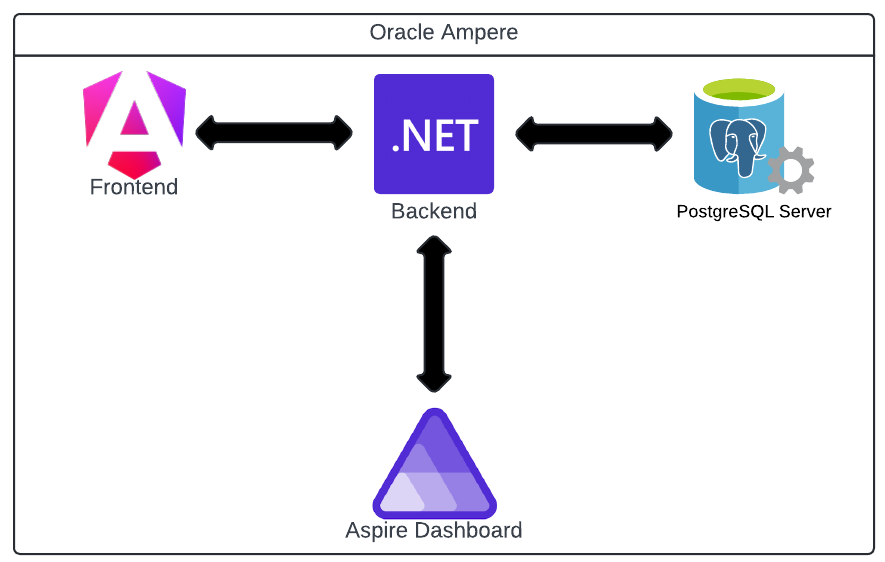
\includegraphics[width=1\textwidth]{attachments/arch-diag}
    \caption{Diagram systemu w środowisku docelowym}
    \label{fig:figure}
\end{figure}

\pagebreak
\subsection{Konfiguracja Nginx}
\label{subsec:konfiguracja-nginx}
Przedstawiona poniżej konfiguracja serwera NGINX zawiera definicje kilku serwerów wirtualnych dla różnych domen i usług.
Zamieszczono w niej szczegółowe wyjaśnienie każdego elementu konfiguracji.

\subsubsection{Główny serwer obsługujący \texttt{city-planner.budziszm.pl}}
\begin{minipage}{\linewidth}
\begin{lstlisting}[label={lst:n1}]
server {
  server_name city-planner.budziszm.pl;

  root /var/www/city-planner.budziszm.pl/html;

  index index.html;
\end{lstlisting}
\end{minipage}
\begin{itemize}
    \item \texttt{server\_name city-planner.budziszm.pl;}: Określa nazwę serwera, który obsługuje tę konfigurację.
    \item \texttt{root /var/www/city-planner.budziszm.pl/html;}: Ustala katalog główny dla plików serwowanych przez ten serwer.
    \item \texttt{index index.html;}: Ustawia domyślny plik indeksu.
\end{itemize}

\begin{minipage}{\linewidth}
\begin{lstlisting}[label={lst:n2}]
  location = /favicon.ico { access_log off; log_not_found off; }
\end{lstlisting}
\end{minipage}
\begin{itemize}
    \item \texttt{location = /favicon.ico}: Reguła dla \texttt{favicon.ico}.
    Wyłącza logowanie dostępu oraz błędów, jeśli plik nie zostanie znaleziony.
\end{itemize}

\subsubsection{Konfiguracja gzip}
\begin{minipage}{\linewidth}
\begin{lstlisting}[label={lst:n3}]
  gzip on;
  gzip_static on;
  gzip_types
    text/plain
    text/css
    text/js
    text/xml
    text/javascript
    application/javascript
    application/json
    application/xml
    application/rss+xml
    image/svg+xml;
  gzip_proxied no-cache no-store private expired auth;
\end{lstlisting}
\end{minipage}
\begin{itemize}
    \item \texttt{gzip on;} i \texttt{gzip\_static on;}: Włącza kompresję gzip i kompresję statyczną.
    \item \texttt{gzip\_types}: Określa typy MIME, które mają być kompresowane.
    \item \texttt{gzip\_proxied}: Definiuje warunki, pod którymi odpowiedzi z proxy mogą być kompresowane.
\end{itemize}

\subsubsection{Konfiguracja cache dla CSS i JS}
\begin{minipage}{\linewidth}
\begin{lstlisting}[label={lst:n4}]
  location ~*.(css|js)$ {
    add_header Cache-Control "public, immutable, max-age=31536000";
  }
\end{lstlisting}
\end{minipage}
\begin{itemize}
    \item \texttt{location ~*.(css|js)\$}: Obsługuje wszystkie pliki CSS i JS@.
    \item \texttt{add\_header Cache-Control "public, immutable, max-age=31536000";}: Dodaje nagłówek kontrolujący cache, który umożliwia przechowywanie plików w pamięci podręcznej przez rok.
\end{itemize}

\subsubsection{Przekierowania proxy dla \texttt{/Api} i \texttt{/confirmEmail}}
\begin{minipage}{\linewidth}
\begin{lstlisting}[label={lst:n5}]
  location /Api {
    rewrite /Api/(.*) /$1 break;
    proxy_pass http://localhost:5000;
    proxy_redirect off;
    proxy_set_header Host $host;
  }

  location /confirmEmail {
    proxy_pass http://localhost:5000;
    proxy_redirect off;
    proxy_set_header Host $host;
  }
\end{lstlisting}
\end{minipage}
\begin{itemize}
    \item \texttt{location /Api} i \texttt{location /confirmEmail}: Przekierowują żądania na odpowiednie endpointy do lokalnego serwera działającego na porcie 5000.
\end{itemize}

\subsubsection{Obsługa plików w \texttt{/thesis}}
\begin{minipage}{\linewidth}
\begin{lstlisting}[label={lst:n6}]
  location ~* /thesis/(.*)$ {
    root /opt/city-planner-documentation;
    rewrite /thesis/(.*) /$1.pdf break;
    add_header Content-Disposition 'inline';
    try_files $uri =404;
  }

  location /thesis {
    root /opt/city-planner-documentation;
    rewrite /thesis /thesis.pdf break;
    add_header Content-Disposition 'inline';
    try_files $uri =404;
  }
\end{lstlisting}
\end{minipage}
\begin{itemize}
    \item Obsługuje dostęp do plików w katalogu \texttt{/opt/city-planner-documentation}, zmieniając ścieżki i dodając nagłówek \texttt{Content-Disposition} do wyświetlania plików PDF w przeglądarce.
\end{itemize}

\subsubsection{Główne ustawienia dla ścieżek i SSL}
\begin{minipage}{\linewidth}
\begin{lstlisting}[label={lst:n7}]
  location / {
    try_files $uri$args $uri$args/ /index.html;
  }

  listen 443 ssl; # managed by Certbot
  ssl_certificate /etc/letsencrypt/live/city-planner.budziszm.pl/fullchain.pem; # managed by Certbot
  ssl_certificate_key /etc/letsencrypt/live/city-planner.budziszm.pl/privkey.pem; # managed by Certbot
  include /etc/letsencrypt/options-ssl-nginx.conf; # managed by Certbot
  ssl_dhparam /etc/letsencrypt/ssl-dhparams.pem; # managed by Certbot
\end{lstlisting}
\end{minipage}
\begin{itemize}
    \item \texttt{location /}: Przekierowuje do pliku \texttt{index.html} jeśli plik lub katalog nie zostaną znalezione.
    \item \texttt{listen 443 ssl;}: Konfiguruje serwer do nasłuchiwania na porcie 443 z SSL\@.
    \item \texttt{ssl\_certificate}, \texttt{ssl\_certificate\_key}, \texttt{include}, \texttt{ssl\_dhparam}: Konfiguracja SSL przy użyciu certyfikatów Let's Encrypt.
\end{itemize}

\subsubsection{Przekierowanie HTTP do HTTPS}
\begin{minipage}{\linewidth}
\begin{lstlisting}[label={lst:n8}]
server {
    if ($host = city-planner.budziszm.pl) {
        return 301 https://$host$request_uri;
    } # managed by Certbot

    server_name city-planner.budziszm.pl;
    listen 80;
    return 404; # managed by Certbot
}
\end{lstlisting}
\end{minipage}
\begin{itemize}
    \item Przekierowuje ruch HTTP na HTTPS dla \texttt{city-planner.budziszm.pl}.
\end{itemize}

\subsubsection{Serwer obsługujący \texttt{logs.city-planner.budziszm.pl}}
\begin{minipage}{\linewidth}
\begin{lstlisting}[label={lst:n9}]
server {
  server_name logs.city-planner.budziszm.pl;
  auth_basic           "Administrator's Area";
  auth_basic_user_file /etc/apache2/.htpasswd;
  error_log  /var/log/nginx/error.log debug;

  location / {
    proxy_pass https://localhost:18888;
    proxy_redirect off;
    proxy_http_version 1.1;
    proxy_set_header Upgrade $http_upgrade;
    proxy_set_header Connection "Upgrade";
    proxy_set_header Host $host;
  }

  listen 443 ssl; # managed by Certbot
  ssl_certificate /etc/letsencrypt/live/city-planner.budziszm.pl/fullchain.pem; # managed by Certbot
  ssl_certificate_key /etc/letsencrypt/live/city-planner.budziszm.pl/privkey.pem; # managed by Certbot
  include /etc/letsencrypt/options-ssl-nginx.conf; # managed by Certbot
  ssl_dhparam /etc/letsencrypt/ssl-dhparams.pem; # managed by Certbot
}
\end{lstlisting}
\end{minipage}
\begin{itemize}
    \item Obsługuje ruch na \texttt{logs.city-planner.budziszm.pl} z podstawową autoryzacją.
    \item Przekierowuje ruch do lokalnego serwera na porcie 18888 z obsługą WebSocketów.
\end{itemize}

\subsubsection{Przekierowanie HTTP do HTTPS dla \texttt{logs.city-planner.budziszm.pl}}
\begin{minipage}{\linewidth}
\begin{lstlisting}[label={lst:n10}]
server {
    if ($host = logs.city-planner.budziszm.pl) {
        return 301 https://$host$request_uri;
    } # managed by Certbot

    listen 80;
    server_name logs.city-planner.budziszm.pl;
    return 404; # managed by Certbot
}
\end{lstlisting}
\end{minipage}
\begin{itemize}
    \item Przekierowuje ruch HTTP na HTTPS dla \texttt{logs.city-planner.budziszm.pl}.
\end{itemize}

\subsubsection{Mapowanie nagłówka \texttt{Connection} w zależności od nagłówka \texttt{Upgrade}}
\begin{minipage}{\linewidth}
\begin{lstlisting}[label={lst:n11}]
map $http_upgrade $connection_upgrade {
  default upgrade;
  ''      close;
}
\end{lstlisting}
\end{minipage}
\begin{itemize}
    \item Ustawia wartość nagłówka \texttt{Connection} w zależności od obecności nagłówka \texttt{Upgrade}.
    Umożliwia to poprawne działanie WebSocketów.
\end{itemize}

Ta konfiguracja zapewnia pełną obsługę zarówno dla serwowania statycznych stron, jak i przekierowania ruchu do usług backendowych, zapewniając jednocześnie bezpieczeństwo przez użycie SSL i kontrolę cache dla plików statycznych.

\subsection{Deployment backendu}
\label{subsec:deployment-backendu}
Ten skrypt Bash wykonuje kilka kroków, aby wdrożyć backend aplikacji.
Poniżej znajduje się szczegółowy opis, co robi każda jego część:

\subsubsection{Usuwanie wszystkich plików z /opt/city-planner-backend/publish}
Ten krok usuwa wszystkie pliki z katalogu \texttt{/opt/city-planner-backend/publish}, aby przygotować miejsce na nowe pliki.
\begin{minipage}{\linewidth}
\begin{lstlisting}[style=shell-colored,label={lst:db1}]
+echo+ "Removing all files from /opt/city-planner-backend/publish"
+rm -Rf+ /opt/city-planner-backend/publish/*
\end{lstlisting}
\end{minipage}

\subsubsection{Kopiowanie plików do /opt/city-planner-backend/publish/}
Ten krok kopiuje opublikowane pliki z katalogu \texttt{WebApi/bin/production/net8.0/linux-arm64/publish/} do \texttt{/opt/city-planner-backend/publish/}.
\begin{minipage}{\linewidth}
\begin{lstlisting}[style=shell-colored,label={lst:db2}]
+echo+ "Copying publish files to /opt/city-planner-backend/publish/"
+cp+ WebApi/bin/production/net8.0/linux-arm64/publish/* /opt/city-planner-backend/publish/
\end{lstlisting}
\end{minipage}

\subsubsection{Przygotowanie pliku usługi SystemD}
Ten krok tworzy nowy plik usługi SystemD dla backendu aplikacji.
Plik usługi zawiera konfigurację dla SystemD, w tym opis, zależności, ustawienia serwisu i polecenie uruchomienia.

\begin{minipage}{\linewidth}
\begin{lstlisting}[style=shell-colored,label={lst:db3}]
+echo+ "Preparing SystemD service file"
+rm -f+ /etc/systemd/system/city-planner-backend.service
+cat+ <<EOT >> /etc/systemd/system/city-planner-backend.service
[Unit]
Description=City planner backend
After=network.target
StartLimitIntervalSec=0

[Service]
Type=simple
Restart=always
RestartSec=1
User=ubuntu
EnvironmentFile=/opt/city-planner-backend/environment.conf
WorkingDirectory=/opt/city-planner-backend/publish
ExecStart=/opt/city-planner-backend/publish/WebApi

[Install]
WantedBy=multi-user.target
EOT
\end{lstlisting}
\end{minipage}

\subsubsection{Włączanie pliku usługi SystemD}
Ten krok włącza nowo utworzony plik usługi SystemD, aby uruchamiał się automatycznie przy starcie systemu.
\begin{minipage}{\linewidth}
\begin{lstlisting}[style=shell-colored,label={lst:db4}]
+echo+ "Enabling SystemD service file"
+systemctl enable+ city-planner-backend
\end{lstlisting}
\end{minipage}

\subsubsection{Restartowanie usługi SystemD}
Ten krok restartuje usługę SystemD, aby zastosować nowe ustawienia i uruchomić backend aplikacji.
\begin{minipage}{\linewidth}
\begin{lstlisting}[style=shell-colored,label={lst:db5}]
+echo+ "Restarting SystemD service file"
+systemctl restart+ city-planner-backend
\end{lstlisting}
\end{minipage}

\subsubsection{Zakończenie wdrożenia backendu}
Ten krok wyświetla komunikat informujący o zakończeniu wdrożenia backendu.
\begin{minipage}{\linewidth}
\begin{lstlisting}[style=shell-colored,label={lst:db6}]
+echo+ "Backend deployment done"
\end{lstlisting}
\end{minipage}

\subsubsection{Całość kodu}
\begin{minipage}{\linewidth}
\begin{lstlisting}[style=shell-colored,label={lst:db7}]
#!/bin/bash

+echo+ "Removing all files from /opt/city-planner-backend/publish"
+rm -Rf+ /opt/city-planner-backend/publish/*

+echo+ "Copying publish files to /opt/city-planner-backend/publish/"
+cp+ WebApi/bin/production/net8.0/linux-arm64/publish/* /opt/city-planner-backend/publish/
+echo+ "Preparing SystemD service file"
+rm -f+ /etc/systemd/system/city-planner-backend.service
+cat+ <<EOT >> /etc/systemd/system/city-planner-backend.service
[Unit]
Description=City planner backend
After=network.target
StartLimitIntervalSec=0

[Service]
Type=simple
Restart=always
RestartSec=1
User=ubuntu
EnvironmentFile=/opt/city-planner-backend/environment.conf
WorkingDirectory=/opt/city-planner-backend/publish
ExecStart=/opt/city-planner-backend/publish/WebApi

[Install]
WantedBy=multi-user.target
EOT

+echo+ "Enabling SystemD service file"
+systemctl enable+ city-planner-backend
+echo+ "Restarting SystemD service file"
+systemctl restart+ city-planner-backend

+echo+ "Backend deployment done"
\end{lstlisting}
\end{minipage}
